\newpage
\subsection{Ungedämpfte Schwingungen}
\textbf{Harmonische Schwingung 1}\\
Eine harmonische Schwingung ist durch folgende Anfangsbedingungen gegeben: Die Auslenkung $A=2cm$ zum Zeitpunkt $t = 0$s. Die Geschwindigkeit $u_0 = -2cm$ zum Zeitpunkt $t = 0$. Die Schwingung hat eine Periode $T=2s$. Durch diese Angaben ist der weitere Verlauf
der Schwingung eindeutig bestimmt. Berechnen Sie die harmonische Funktion, die diese Schwingung beschreibt.

\begin{align*}
y(0) &=s_0 =  2cm\quad \dot{y}(0) = u_0 = -2cm\\
y(t = 0) &= A \cdot \sin(\omega \cdot 0 + \varphi) = s_0\\
\dot{y}(t = 0) &= \omega \cdot  A \cdot \cos(\omega \cdot 0 + \varphi) = v_0\\
A\cdot \sin(\varphi) &= s_0\\
A\cdot \cos(\varphi) &=\frac{v_0}{\omega}\\
&\textrm{ 2 Gleichungen} \Rightarrow \textrm{ solve!}
\end{align*}

\textbf{Mathematisches Pendel}\\
Die an einem Baukran knapp über dem Boden hängende Last pendelt langsam hin und her. Eine Schwingung dauert 15.6 s. Wie hoch ist der Kran?
\[
	T= 2\pi\sqrt{\frac{l}{g}}\Rightarrow l=\frac{gT^2}{4\pi^2} = \frac{9.81\cdot (15.6s)^2}{4\pi^2} = 60.47m
\]

\subsection{Gedämpfte Schwingungen}
\textbf{1. Logarithmisches Dekrement}\\
Wie gross ist das logarithmische Dekrement der gedämpften harmonischen Schwingung eines Massenpunktes, wenn dieser in $10s$ $50\%$ seiner mechanischen Energie verliert und die Schwingungsdauer $0.2s$ beträgt?
\begin{align*}
	\frac{E_2}{E_1} &= \frac{(A_2)^2}{(A_1)^2} = 0.5\\
	A_1&=\sqrt{2}\cdot A_2\\
	\frac{A_1}{A_2} &= \sqrt{2}=e^{\delta t}\\
	\delta \cdot t&= \ln(\sqrt{2})\\
	\Lambda&=\delta T = \frac{\ln(\sqrt{2})\cdot T}{t}=\frac{\ln(2)\cdot 0.2s}{10s}=6.93\cdot 10^{-3}
\end{align*}

\textbf{2. Logarithmisches Dekrement}\\
Das logarithmische Dekrement einer gedämpften Schwingung beträgt $\Lambda = 1.1$. Um wieviel unterscheidet sich die Eigenfrequenz der gedämpften Schwingung von der ungedämpften Schwingung?
\begin{align*}
\delta &= \frac{\Lambda}{T}\\
\omega&=\sqrt{\omega_0^2-\delta^2}=\sqrt{\left(\frac{2\pi}{T}\right)^2-\left( \frac{\Lambda}{T}\right)^2}\\
\frac{\omega}{\omega_0}&= \frac{\frac{2\pi}{T}}{\sqrt{\left(\frac{2\pi}{T}\right)^2-\left(\frac{1.1}{T} \right)^2}} = 1.01568\\
\%&= ans\cdot 100\%-100\% = 1.568\%
\end{align*}






\subsection{Motor mit Unwucht}
\begin{minipage}{0.49\textwidth}
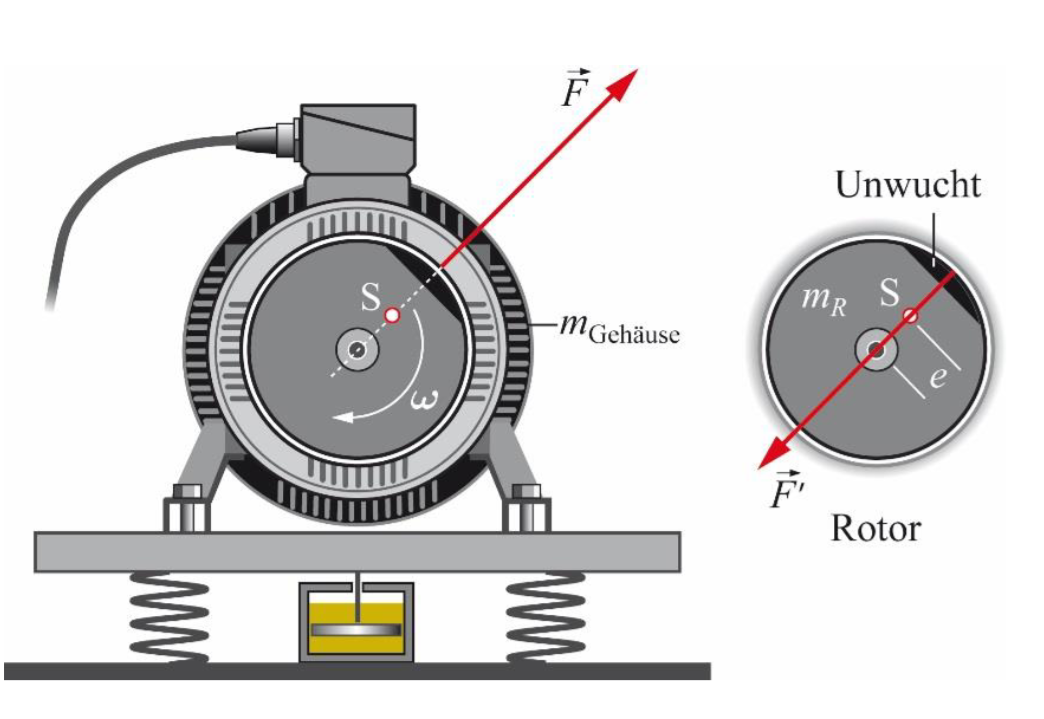
\includegraphics[width=0.8\textwidth]{bilder/motor_unwucht.png}
\end{minipage}
\begin{minipage}{0.49\textwidth}
\begin{align*}
D&=0.1\\
M_{tot} &= 300kg\\
m&= 30kg\\
M&= 270kg\\
f_e&= \textrm{ Kraft zwischen Rotor und Stator}\\
e&= 5mm = \textrm{Exzentrizität}\\
\omega  &= 2\pi f = \frac{2\pi\cdot 1500}{60\frac{s}{min}} = 50\frac{\pi}{s} = 157.08\\
k&= 500\frac{N}{cm} = 50'000\frac{N}{m}
\end{align*}
\end{minipage}

\[
	\begin{array}{rll}
		I&M\ddot{y} &= -k y -b\dot{y} +f_e\\
		II&m(\ddot{y}-\omega^2 e\cdot\sin(\omega t))&=-f_e\\
		I+II&(M+m)\ddot{y} - me\omega^2 \cdot \sin(\omega t) &=-ky-b\dot{y}\\
		& M_{tot} \ddot{y} +b\dot{y} + ky &= m e\omega^2 \cdot \sin(\omega t)\qquad \qquad \textrm{Standartlösung}\\
		&\omega_0 &=\sqrt{\frac{k}{M_{tot}}} = \sqrt{\frac{50'000}{300}} = 12.9\frac{rad}{s}\\
		&f_0 = \frac{\omega_0}{2\pi} = 2.05\frac{1}{s}&f_m = \frac{1500}{60} = 25\frac{rad}{s}	\\
		&\eta = \frac{\omega}{\omega_0} = \frac{157.08}{2.05} = 12.17\\
		&F_0=\underset{\textrm{Kraft Boden ohne Federn}}{m\cdot e\cdot \omega^2}  &= 30kg\cdot 0.005m\cdot (157.08)^2 = 3701N\\[1em]
		\textrm{Oder gemäss \ref{Unwucht} S. \pageref{Unwucht}}& F_{B0}=\dfrac{m_R\,e\,\omega^2\,\sqrt{1+4D^2\eta^2}}{\sqrt{(1-\eta^2)^2+4D^2\eta^2}}\\
		&=\frac{30kg\cdot 0.005\cdot (157.08)^2\cdot \sqrt{1+4\cdot 0.1^2\cdot 12.17^2}}{\sqrt{(1-12.17^2)^2+4\cdot 0.1^2\cdot 12.17^2}} &= 65.76N
	\end{array}
\]


\subsection{Gleichmässig beschleunigte Masse an Feder}
Eine Masse mit der Masse $m=0.1kg$ hängt an einer ungespannten Feder der Länge $l=0.5m$ mit der Federkonstante $k=10N/m$. Zum Zeitpunkt $t=0$ beschleunigt der Aufhängepunkt der Feder mit einer Konstanten Beschleunigung $a=2m/s$ nach oben.
\begin{align*}
	y(0) &=\frac{-mg}{k} = \frac{-0.1\cdot 9.81}{k} = -0.0981m\\
	\dot{y}(0) &= 0\\
	m\cdot \ddot{y}+k\cdot y &= 0 \Rightarrow y_H = A\cdot \sin(\omega t +\varphi)\\
	m\cdot \ddot{y}+k\cdot y &=\frac{1}{2} a t^2-mg\qquad \textrm{ Ansatz:}\quad yp=c_0+c_1\cdot t +c_2\cdot t^2\\
	\textrm{eingesetzt }\quad &2\cdot m\cdot c_2+k(c_0+c_1\cdot t +c_2\cdot t^2)=k\cdot \frac{1}{2}\cdot a\cdot t^2 -m\cdot g\\
	\textrm{Koeffizientenvergleich}\quad &k\cdot c_2 = \frac{1}{2} \cdot k\cdot a\\
	&c_2 = \frac{a}{2}\\
	&c_1=0\\
	&2m\cdot c_2+k\cdot c_0 = -m\cdot g\\
	&c_2 =\frac{-m\cdot g}{k}-\frac{m\cdot a}{k}\\
	\textrm{eingesetzt}\quad &y(t) = A\cdot \sin(\omega t +\varphi) -\frac{mg}{k}-\frac{ma}{k}+\frac{a}{2} t^2\\
	\textrm{Anfangswerte:}\quad t=0\quad &A\sin(\varphi) -\frac{mg}{k}-\frac{ma}{k} = \frac{-mg}{k}\\
	&A\sin(\varphi) = \frac{ma}{k}\Rightarrow A=\frac{ma}{k}\\
	&A\omega \cos (\omega t+\varphi) = 0 \Rightarrow \varphi = \frac{\pi}{2}\\
	y(t) &=0.02\sin\left(\frac{1}{10}t+\frac{\pi}{2}\right)-1.181+t^2
\end{align*}